
\documentclass[journal]{IEEEtran}
    \usepackage[spanish]{babel}
    \selectlanguage{spanish}
    \usepackage[utf8]{inputenc}
    \usepackage{hyperref}
    \usepackage{lipsum}

    % *** GRAPHICS RELATED PACKAGES ***
    %
    \ifCLASSINFOpdf
    \usepackage[pdftex]{graphicx}
    \DeclareGraphicsExtensions{.pdf,.jpeg,.png}
    \else

    \fi

    \usepackage{booktabs}
    \usepackage{tikz}
    \def\checkmark{\tikz\fill[scale=0.4](0,.35) -- (.25,0) -- (1,.7) -- (.25,.15) -- cycle;} 

    % *** MATH PACKAGES ***
    %
    \usepackage{amsmath}
    \usepackage{amsfonts}
    \interdisplaylinepenalty=2500

    \usepackage{array}
    \usepackage{fixltx2e}
    \usepackage{stfloats}
    \usepackage{booktabs}
    \usepackage{subcaption}

    % *** PDF, URL AND HYPERLINK PACKAGES ***
    %
    \usepackage{url}

    % correct bad hyphenation here
    \hyphenation{op-tical net-works semi-conduc-tor}


\begin{document}

    \title{Reinforcement Learning:\\ FlappyBird}

    \author{Kenneth Obando Rodríguez,~\IEEEmembership{Instituto Tecnológico de Costa Rica}\\
                Alejandro Pacheco Quesada,~\IEEEmembership{Instituto Tecnológico de Costa Rica}}

        % The paper headers
    \markboth{Inteligencia Artificial, Mayo~2018}%
        {Shell \MakeLowercase{\textit{et al.}}: Bare Demo of IEEEtran.cls for IEEE Journals}

        % make the title area
    \maketitle

    
% :::::::::::::::::::::::
%     ABSTRACT
% :::::::::::::::::::::::
\begin{abstract}

\end{abstract}

% Note that keywords are not normally used for peerreview papers.
\begin{IEEEkeywords}
neural network, gradient descent, softmax, cross-entropy, relu, mnist, machine learning, image classification
\end{IEEEkeywords}

\IEEEpeerreviewmaketitle


\section{Introducción}
    \IEEEPARstart{E}{xisten} problemas computacionales que requieren que un programa realice una acción ante un estado determinado, con la agravante que estos estados pueden tener muchas variables diferentes que lo convierten en una tarea prácticamente imposible para una aproximación estática de la solución. Ante estos problemas, surge toda una rama del campo de la Inteligencia Artificial que se llama Aprendizaje Por Reforzamiento \emph{(``Reinforcement Learning'')}, que consiste, en términos generales, en entrenar un algoritmo utilizando premios \emph{(``reward''))} positivos o negativos, según sea el resultado de la acción tomada en un estado dado.

    Esta investigación tiene como objetivo implementar un algoritmo de \emph{Reinforcement Learning} conocido como ``Policy Gradient'' para entrenar un modelo computacional para que juegue con éxito ``FlappyBird'', para ello se utilizan herramientas como PyTorch, 
 

\section{Trabajo relacionado}
    Un dato interesante es que el famoso visionario Turing (1948,1950) propuso una aproximación del aprendizaje por reforzamiento aunque no estaba totalmente convencido de su efectividad: \emph{``... el uso de castigos y premios puede, en el mejor de los casos, ser parte de un proceso de enseñanza.''} \cite{Turing1948,Turing1950}. Se sospecha que la primera investigación exitosa en este campo es la de Arthur Samuel, el cual contiene una buena parte de las ideas modernas en parendizaje por reforzamiento, incluyendo la aproximación utilizando una función \cite{Rusell2010}.

    Desde principios de la década de los 90 se realizaron aportes en el campo del aprendizaje por reforzamiento utilizando \emph{``Policy Gradient''} inicialmente gracias a Ronald Williams que desarrolló esta familia de algoritmos. Trabajos posteriores hicieron grandes aportes, aunque fue con Papavassiliou y Russel que se describe un nuevo tipo de reforzamiento que converge con cualquier tipo de aproximador de función \cite{Papavassiliou1999}. A partir de estos estudios, se han hecho bastantes aproximaciones, y se ha llevado a una rápida y amplia implementación gracias a herramientas como PyTorch, TensorFlow y hardware como las GPU mediante librerías como CUDA.

    Una buena síntesis sobre los métodos que existen actualmente en Policy Gradient se encuentra en \cite{Peters2010}.

\section{Metodología}
    En términos generales, este proyecto se divide en diferentes etapas para el entrenamiento del modelo computacional: FlappyBird contiene toda la lógica del juego, el renderizado de las imágenes y recibe las acciones del agente; la etapa de preprocesamiento, la Red Convolucional y los reportes mediante gráficos e imágenes generadas utilizando la herramienta PLT.
\subsection{Juego: FlappyBird}
    FlappyBird es un juego que consiste en hacer que un ave pase en medio de una serie de dos tuberías que se van aproximando constantemente, para ello, el jugador debe apretar una tecla (normalmente \emph{``espacio''}) que provoca que el pájaro salte en el aire. El jugador debe ser lo suficientemente hábil para coordinar los saltos, la distancia y el tiempo. 

    Este juego contiene características especiales que permiten ser un candidato para ser utilizado para entrenar un agente mediante Aprendizaje por Reforzamiento: 
    \begin{itemize}
        \item Sólo requiere dos acciones de parte del agente: saltar o no realizar ninguna acción.
        \item El agente sólo debe preocuparse por la ubicación del pájaro y la cercanía de las tuberías más próximas. 
        \item Las figuras de las imágenes son sencillas, con colores sólidos, lo que facilita la etapa de preprocesamiento.
    \end{itemize}

\subsection{Preprocesamiento}
    Para facilitar la etapa de aprendizaje, se realiza un preprocesamiento de cada imagen generada por el juego, el cual consiste en aplicar un filtro a una capa del espectro visual. Mediante diferentes pruebas realizadas, se comprobó que en la capa verde los elementos importantes para el aprendizaje \emph{``el pájaro y las tuberías''} mantienen una tonalidad semejante, lo que permite filtrar por los valores de esta tonalidad con un costo computacional mínimo. Además, se recorta las secciones de la imagen que no tienen un valor significativo para el aprendizaje. En la figura~\ref{fig:preproc} se puede apreciar las diferentes etapas del preprocesamiento.

    \begin{figure}[h]
        \centering
        %add desired spacing between images, e. g. ~, \quad, \qquad, \hfill etc. 
        %(or a blank line to force the subfigure onto a new line)
        \begin{subfigure}[b]{0.5\textwidth}
            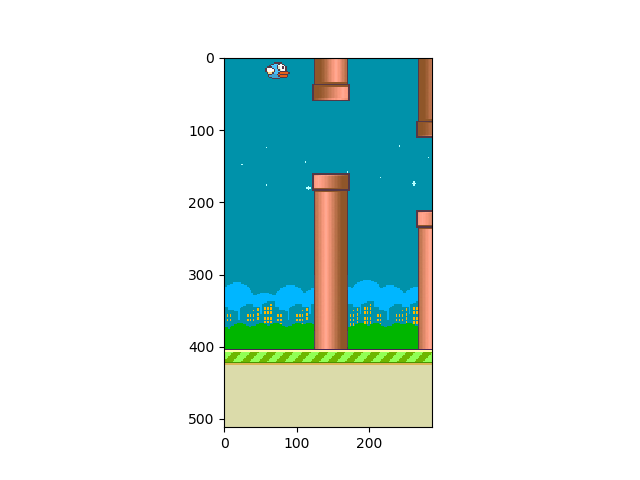
\includegraphics[width=\textwidth]{images/pre1.png}
            \caption{}
        \end{subfigure}
        ~
        \begin{subfigure}[b]{0.5\textwidth}
            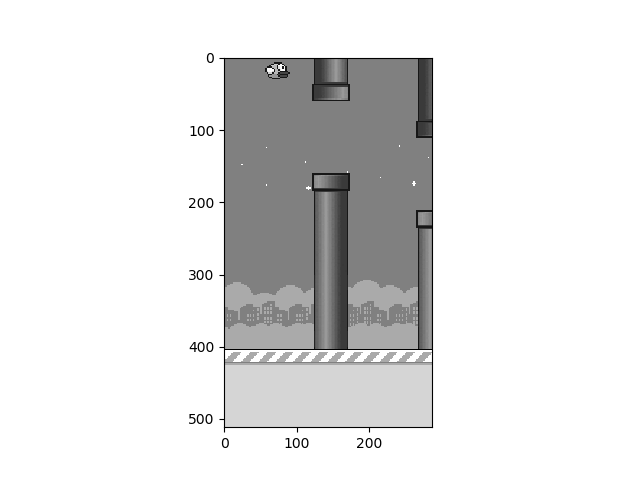
\includegraphics[width=\textwidth]{images/pre2.png}
            \caption{}
        \end{subfigure}
        \begin{subfigure}[b]{0.5\textwidth}
            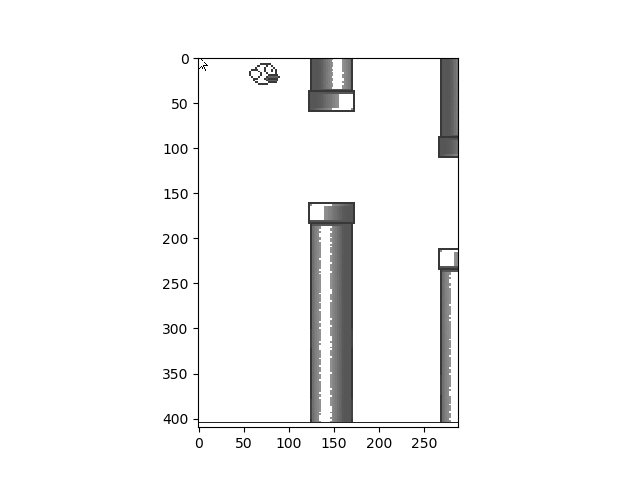
\includegraphics[width=\textwidth]{images/pre3.png}
            \caption{}
        \end{subfigure}
        \caption{Imágenes las diferentes etapas del preprocesamiento: (a) Imagien inicial; (b) Capa del espectro verde; (c) Imagen con el filtro y el recorte aplicado \label{fig:animals}}
    \end{figure}

\subsection{Red Neuronal}
Para esta investigación se utilizó una red convolucional, que de base para los experimentos tiene tres capas, cada una con una capa de \emph{``MaxPooling''}, la última capa es una red neuronal \emph{``FullyConnected''} con una salida con SoftMax. Las características de cada capa se detallan en el Cuadro~\ref{tab:convDescrip}. Cabe decir que, como parte de la experimientación, se probó con varias convinaciones de red convolucional para comprobar los resultados.

\begin{table*}[]
    \centering
    
    \begin{tabular}{llllll}
        \hline
        \textbf{Capa} & \textbf{Descripción} & \textbf{\begin{tabular}[c]{@{}l@{}}Cantidad \\ de Kernels\end{tabular}} & \textbf{\begin{tabular}[c]{@{}l@{}}Tamaño \\ del Kernel\end{tabular}} & \textbf{Stride} & \textbf{Activación} \\ \hline
        1  & Convolucional        & 10    & 5     & 1     & ReLu   \\
        2  & MaxPooling           & N/A   & 2     & 1     & N/A    \\
        3  & Convolucional        & 12    & 7     & 1     & ReLu   \\
        4  & MaxPooling           & N/A   & 2     & 1     & N/A    \\
        5  & Convolucional        & 12    & 7     & 1     & ReLu   \\
        6  & MaxPooling           & N/A   & 2     & 1     & N/A    \\
        7  & DropOut              & N/A   & N/A   & N/A   & N/A    \\
        8  & Red Fully Connected  & N/A   & N/A   & N/A   & N/A    \\ \hline
    \end{tabular}
    \caption{Descripción de las capas de la Red Convolucional.\label{tab:convDescrip}}
    
    \end{table*}


\subsection{Entrenamiento y testing}


\subsection{Red neuronal}

\section{Experimentos}
En esta secci´on describen los experimentos ejecutados para
evaluar el aprendizaje que tiene el agente bajo diversos escenarios.
\subsection{}
Con este experimento se pretende evaluar como se vería afectado el aprendizaje del agente al utilizar diferentes cantidades de capas de convolucion, diferente cantidad de \emph{kernels} y varios tamanos de \emph{kernels}. Para todos los experimentos se utilizó únicamente una capa \emph{fully-connected}, con dos neuronas de salida. Además, se especifica en cuales capas se aplicó \emph{dropout} y el tamano del \emph{window} utilizado para hacer \emph{pooling} a cada capa.

\subsection{Preprocesamiento de los datos de entrada}
Para evaluar los experimentos especificados anteriormente, el conjunto de datos a utilizar serán los estados proporcionados por el entorno donde se encuentra el agente. Se pretende realizar los experimeintos con preprocesamientos de los datos y si el preprocesamiento.

\begin{table}[h!]
    \centering
    
    \begin{tabular}{@{}lllll@{}}
        \toprule
        Capa & Dropout & \textbf{\begin{tabular}[c]{@{}l@{}}Cantidad \\ de Kernels\end{tabular}} & Tamaño del Kernel & Pooling Window \\ \midrule
        1    & No      & 10                  & 5                 & 7              \\
        2    & Sí      & 12                  & 7                 & 5              \\
        3    & No      & 16                  & 11                & 3              \\ \bottomrule
    \end{tabular}
    \caption{Experimento A1, con 3 capas.\label{tab:A1}}
    \end{table}


    \begin{table}[h!]
        \centering
        
        \begin{tabular}{@{}lllll@{}}
            \toprule
            Capa & Dropout & \textbf{\begin{tabular}[c]{@{}l@{}}Cantidad \\ de Kernels\end{tabular}} & Tamaño del Kernel & Pooling Window \\ \midrule
            1    & No      & 6                   & 11                & 7             \\
            1    & No      & 10                  & 5                 & 7              \\
            2    & Sí      & 12                  & 7                 & 5              \\
            3    & No      & 16                  & 11                & 3              \\ \bottomrule
        \end{tabular}
        \caption{Experimento A1, con 3 capas.\label{tab:A1}}
        \end{table}
    
        \begin{table}[h!]
            \centering
            \begin{tabular}{@{}lllll@{}}
                \toprule
                Capa & Dropout & Cantidad de Kernels & Tamaño del Kernel & Pooling Window \\ \midrule
                1    & No      & 6                   & 11                & 7             
            \end{tabular}
            \caption{Experimento A2, con 1 capa.\label{tab:A2}}
            \end{table}
    
        \begin{table}[h!]
            \centering
            \begin{tabular}{@{}lllll@{}}
                \toprule
                Capa & Dropout & Cantidad de Kernels & Tamaño del Kernel & Pooling Window \\ \midrule
                1    & No      & 6                   & 5                 & 7              \\
                2    & Sí      & 8                   & 7                 & 5              \\
                3    & No      & 12                  & 9                 & 3              \\
                4    & Sí      & 12                  & 11                & 3              \\
                5    & No      & 6                   & 11                & 3              \\ \bottomrule
            \end{tabular}
            \caption{Experimento A3, con 5 capas.\label{tab:A3}}
            \end{table}

    \subsubsection{Datos sin preprocesar:} Corresptonde a los datos originales proporcionados por el entorno. Cada imagen tiene las siguientes características:
    \begin{itemize}
        \item Tamaño de $512\times288$ píxeles.
        \item Tiene tres canales de color (RGB).
    \end{itemize}

    \begin{table}[h!]
        \centering
        \begin{tabular}{@{}lllll@{}}
            \toprule
            Capa & Dropout & \textbf{\begin{tabular}[c]{@{}l@{}}Cantidad \\ de Kernels\end{tabular}} & Tamaño del Kernel & Pooling Window \\ \midrule
            1    & No      & 6                   & 5                 & 7              \\
            2    & Sí      & 8                   & 7                 & 5              \\
            3    & No      & 12                  & 9                 & 3              \\
            4    & Sí      & 12                  & 11                & 3              \\
            5    & No      & 6                   & 11                & 3              \\ \bottomrule
        \end{tabular}
        \caption{Experimento A3, con 5 capas.\label{tab:A3}}
        \end{table}

    \subsubsection{Datos preprocesados:} Se pretende realizar algunos ajustes a losdatos originales con el fin de verificar si el modelo aprende más rápido. Cada imagen quedaría con las siguientes características:
    \begin{itemize}
        \item Tamaño de $410\times288$ píxeles.
        \item Tiene tres canales de color (escala de grises).
    \end{itemize}

\subsection{Un experimento que se les ocurra}


\bibliographystyle{IEEEtran}
\bibliography{library}


\section*{Anexos}

    


\end{document}


